\documentclass{article}
\usepackage[a4paper, total={6.5in, 9in}]{geometry}
\usepackage{amsmath}
\usepackage{amssymb}
\usepackage{graphicx}
\usepackage{subfigure}
\usepackage{hyperref}
\usepackage{booktabs}
\usepackage{authblk}
\renewcommand{\labelenumi}{(\alph{enumi})}
\title{CSCI-SHU 360 Machine Learning\\
    Solution to homework 2}
\author{Josiah Li \texttt{yl11912@nyu.edu}}

\begin{document}
    \maketitle
\section{Linear Regression and Convexity}
We have:
\begin{align*}
    L(w) &= (y - Xw)^T (y - Xw)\\
        &= y^Ty - w^TX^Ty - y^TXw+w^TX^TXw.
\end{align*}
We take the directional derivative on direction $ v $:
\begin{align*}
    D_vL(w) &= \lim_{h\to 0 } \frac{L(w+hv) - L(w )}{h}\\
            &=\lim_{h\to 0 } \frac{y^Ty - (w+hv)^TX^Ty - y^TX(w+hv)^TX^TX(w+hv)-y^Ty + w^TX^Ty + y^TXw - w^TX^TXw}{h}\\
            &= -v^TX^Ty - y^TXv + v^TX^TXw +W^TX^TXv\\
            &= v^T \cdot (2X^TXw - 2X^Ty)\\
            &= <v, 2X^TXw - 2X^T y>.
\end{align*}
Thus, the derivative is $\nabla_w L(w) = 2X^TXw - 2X^Ty $.\\
The second order derivative of $ L(w) $ is $ (\nabla_w)^2 L(w) = 2X^TX \geq 0 $.\\
Thus, the loss function is convex as the second order derivative of the function is PSD.
\clearpage
\section{Gaussian Distribution and the Curse of Dimensionality}
\subsection{}
For $ m = 2 $, we have:\\
\begin{align*}
    S_1(r) &= 2\pi r\\
    V_2 (r)&= \pi r^2.
\end{align*}
And for $ m = 3 $, we have:\\
\begin{align*}
    S_2(r) &= 4\pi r^2\\
    V_3(r)&= \frac{4}{3} \pi r^3
\end{align*}
\subsection{}
When $ m \in {2, 3} $, this equation holds: $ 2\pi r = \frac{d}{dr}(\pi r^2) $, $ 4\pi r^2 = \frac{4}{3}\pi r^3 $.\\
Intuitively, we can consider the surface area to be $ \lim_{\Delta r\to 0} \dfrac{V_m(r+\Delta r) - V_m(r)}{\Delta r} $.  $ V_m(r + \Delta r) - V_m(r)  $ can be considered as a shell outside the origin volume with the shell thickness be $ \Delta r $, thus, when the $ \Delta r\to 0 $, the shell goes to the surface of the sphere.
\subsection{}
As $ \bar S_{m-1} $ contains the dimensional information about the sphere (per say, the constant value). What we need to care is the influence of $ r $ and $ m $. Thus $ S_{m - 1}(r) = \bar S_{m - 1} r^{m - 1} $
\subsection{}
We have:\\
\begin{align*}
    p(x) = \frac{1}{(2\pi \sigma ^2 )^{m/2}}\exp \left(-\frac{\Vert x\Vert^2}{2\sigma ^ 2}\right).
\end{align*}
Then we try to do the integration:
\begin{align*}
    \rho_m(r) = \displaystyle\int_{}^{}p(x)dx = \displaystyle\int_{}^{}\frac{1}{(2\pi \sigma ^2 )^{m/2}}\exp \left(-\frac{\Vert x\Vert^2}{2\sigma ^ 2}\right)dx.
\end{align*}
As we have $ \Vert x \Vert = r $, we can get:\\
\begin{align*}
    \rho_m(r) &= \displaystyle\int_{}^{}p(x)dx = \displaystyle\int_{}^{}\frac{1}{(2\pi \sigma ^2 )^{m/2}}\exp \left(-\frac{\Vert x\Vert^2}{2\sigma ^ 2}\right)dx\\
              &= \displaystyle\int_{}^{}\frac{1}{(2\pi \sigma ^2 )^{m/2}}\exp \left(-\frac{r^2}{2\sigma ^ 2}\right)dx\\
              &= \frac{1}{(2\pi \sigma ^2 )^{m/2}}\exp \left(-\frac{r^2}{2\sigma ^ 2}\right)r^{m-1}\bar S_{m - 1}\\
\end{align*}
\subsection{}
When $ m $ is set, $ \rho_m $ only depend on $ r^{m - 1} $ and $ \exp \left(-\dfrac{r^2}{2\sigma ^ 2}\right) $\\
Thus we can let $ f(r)=r^{m - 1}\exp {(-\dfrac{r^2}{2\sigma^2})} $, and we have:
\begin{align*}
    f'(r) &= (m - 1)r^{m - 2} \exp {(-\dfrac{r^2}{2\sigma^2})} - r^{m} \exp {(-\dfrac{r^2}{2\sigma^2})}\dfrac{1}{\sigma^2}\\
          &= (m - 1 - \frac{r^2 }{\sigma ^2 })r^{m - 2}\exp{(-\frac{r^2 }{2\sigma ^2})}
\end{align*}
Thus, when $ m - 1 - \dfrac{r^2}{\sigma ^2 } = 0 $, the function has the extreme point. \\
Which is $ r = \sqrt{(m - 1)\sigma ^2} $, when $ r\leq \sqrt{(m - 1)\sigma ^2} $, $ f'(r) $ increases, thus, the function has a single maximum value at $ r = \sqrt{(m - 1)\sigma ^2} $, when $ m\to \infty $, $ m - 1 \approx m $, which means for large m, $ \rho_m(r) $ has a single maximum value at $ \hat{r} $ such that $ \hat{r} \approx \sqrt{m} \sigma $.
\subsection{}
In order to derive the the form, we calculate $ \dfrac{\rho_m(\hat r + \epsilon)}{\rho_m(\hat r)} $, which is:
\begin{align*}
    \dfrac{\rho_m(\hat r + \epsilon)}{\rho_m(\hat r)} &=    \frac{\frac{1}{(2\pi \sigma ^2 )^{m/2}}\exp {\left(-\frac{(\hat r + \epsilon )^2}{2\sigma ^2}\right)}(\hat r + \epsilon )^{m - 1}\bar S_{m - 1}}{\frac{1}{(2\pi \sigma ^2 )^{m/2}}\exp {\left(-\frac{(\hat r)^2}{2\sigma ^2}\right)}(\hat r )^{m - 1}\bar S_{m - 1}}\\
                                                      &= \left(1 + \frac{\epsilon }{\hat r}\right)^{m - 1}e^{-\dfrac{ 2\hat r \epsilon +  \epsilon ^2}{2\sigma^2}}\\
\end{align*}
In order to get the form we desired, we construct $ \left(1 + \dfrac{\epsilon }{\hat r}\right)^{m - 1} = \exp{((m-1)\ln{(1+\dfrac{\epsilon }{\hat r}))}} $.\\
As we proved in last question, we have $ m = \dfrac{\hat r^2}{\sigma ^2} $. Thus, when for large $ m $, we have $ m - 1 \approx  \dfrac{\hat r^2}{\sigma ^2}  $\\
Thus, we have:\\
\begin{align*}
    \dfrac{\rho_m(\hat r + \epsilon)}{\rho_m(\hat r)} &= \exp\left(\dfrac{\hat r^2}{\sigma ^2}\ln(1+\frac{\epsilon }{\hat r})\right)\exp{\left(-\frac{2\hat r \epsilon  + \epsilon ^2 }{2\sigma^2}\right)}.
\end{align*}
By Taylor Expansion, we have $ \ln(1+\dfrac{\epsilon }{\hat r}) \approx \dfrac{\epsilon }{\hat r} - \dfrac{\epsilon ^2}{2\hat r^2}  $\\
Thus, we can have:\\
\begin{align*}
    \dfrac{\rho_m(\hat r + \epsilon)}{\rho_m(\hat r)} &\approx \exp\left(\frac{\hat r \epsilon }{\sigma ^2 }- \frac{\epsilon ^2 }{2\sigma ^2}\right)\exp{\left(-\frac{2\hat r \epsilon  + \epsilon ^2 }{2\sigma^2}\right)}\\
                                                      &=\exp{\left(-\frac{\epsilon ^2 }{\sigma ^2}\right)}.
\end{align*}
Thus, we have $ \rho{(\hat r +\epsilon )} \approx \rho(\hat r)e^{-\frac{\epsilon ^2 }{\sigma^2}} $.
\subsection{}
We have $ \hat r = \sqrt{m}\sigma \gg \sigma  $ for large m. Thus, most of the sample points reside outside the high dimension sphere with radius $ \sigma $. They are reside on the sphere with raidus $ \hat r \approx \sqrt{m}\sigma  $. As for Low dimensional Gaussian, we have $ \hat r = \sqrt{m-1}\sigma  $. When $ m $ is small, we can see that most of the points reside inside the sphere with radius $ \sigma  $.
\subsection{}
The probability density at the origin will be $ \dfrac{1}{(2\pi \sigma ^2)^ {m/2}} $, and for the point on sphere $ S_{m-1}(\hat r) $, we have $ p = \dfrac{1}{(2\pi \sigma ^2)^ {m/2}} \exp{\left(-\dfrac{\hat r^2}{2\sigma ^2}\right)} $. As this seems to say that the probability on the sphere will be smaller that the origin, but we have to notice that, as $ r $ increases, the volume of the shell will also increase, lead to a balance at $ \hat r $.
\begin{figure}[htbp]
    \begin{center}
        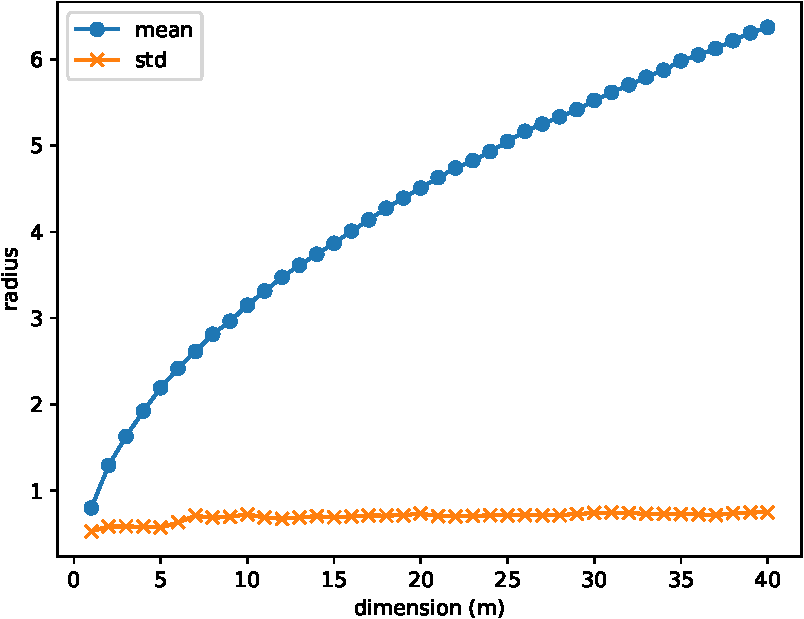
\includegraphics[width=0.5\textwidth]{./figure/mean_std_radius.pdf}
    \end{center}
    \caption{Means and std of radius from m-dimensional Gaussian}\label{fig:}
\end{figure}
\clearpage
\section{Ridge Regression}
\subsection{}
\begin{figure}[htbp]
    \begin{center}
        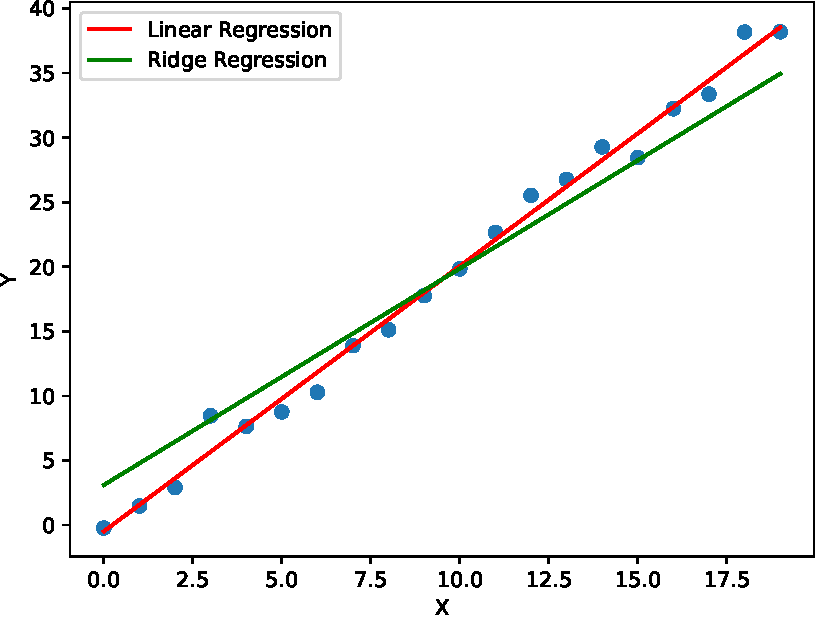
\includegraphics[width=0.5\textwidth]{./figure/ridge_regression.pdf}
    \end{center}
    \caption{Linear regression and ridge regression on datapoints ($ X, y $)}\label{fig:}
\end{figure}
As we can see, in figure 2, standard linear regression has better performance. This is because the linear relation for the datapoints is strong and there are no outliers in this dataset.
\subsection{}
\begin{figure}[htbp]
    \begin{center}
        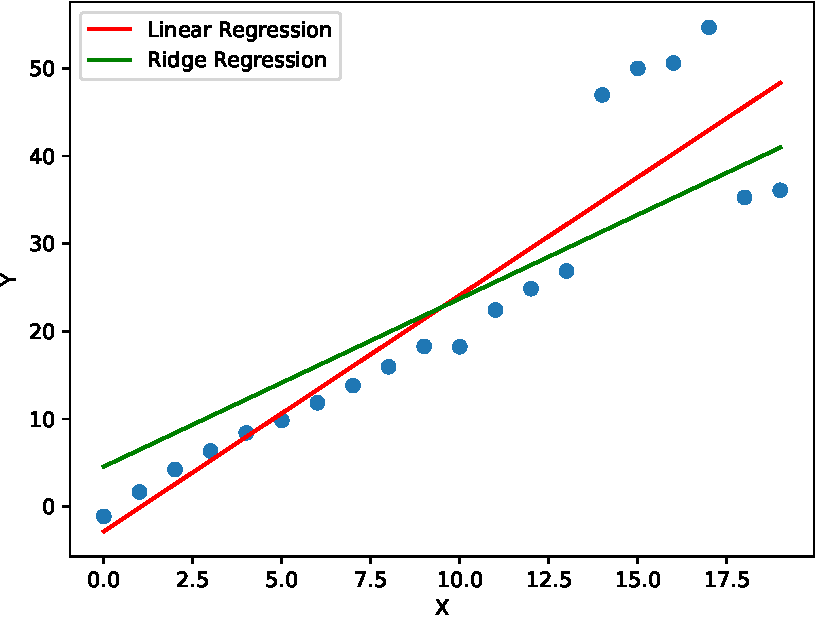
\includegraphics[width=0.5\textwidth]{./figure/ridge_regression_f2.pdf}
    \end{center}
    \caption{Regressions on dataset with outliers}\label{fig:}
\end{figure}
\subsection{}
By taking the derivative of the original target, we have:
\begin{align*}
    D_w F(w) = 2X^TXw - 2y^TX+\eta w
\end{align*}
We have the equation:
\begin{align*}
    2X^TXw - 2y^TX+\eta w &= 0\\
    (2X^TX +\eta) w &= 2y^TX\\
    w&= (X^TX+\frac{\eta}{2}I)^{-1}X^Ty
\end{align*}
\subsection{}
\begin{enumerate}
    \item In this case, we could not compute the closed-form solution. As when we have a $ n\times p  $ matrix and $ p > n $, we can see that after the multiplication we got a $ p\times p $ matrix. The original matrix can have a maximum rank $ n $, leads to a maximum rank $ n $ for $ X^TX $, thus, the new matrix can not be full rank. Which means the new matrix is not invertible.
    \item As we got in the previous question, we have the closed form solution of the ridge regression as:
    \begin{align*}
            w&= (X^TX+\frac{\eta}{2}I)^{-1}X^Ty.
    \end{align*}
    We can notice that, no matter matrix $ X^TX $ is invertible or not, it is always a PSD matrix. Moreover, by the definition of eigenvalue, we have:
    \begin{align*}
        X^TXv &= \lambda v\\
        (X^TX + I)v &= (\lambda + 1) v
    \end{align*}
    Thus, as the origin matrix is PSD ($ \lambda \geq 0 $), we have the eigenvalues for the matrix $ X^TX + I $ always larger than 0. And this ensures that the matrix $ X^TX + I $ is a positive definite matrix. Which means this matrix is always invertible. And we can calculate the closed-form solution solution for ridge regression.
    \clearpage
\end{enumerate}
\section{Programming Problem: Draw an Ellipsoid}\label{sec:Programming Problem: Draw an Ellipsoid} % (fold)
\subsection{}
\begin{figure}[htbp]
    \begin{center}
        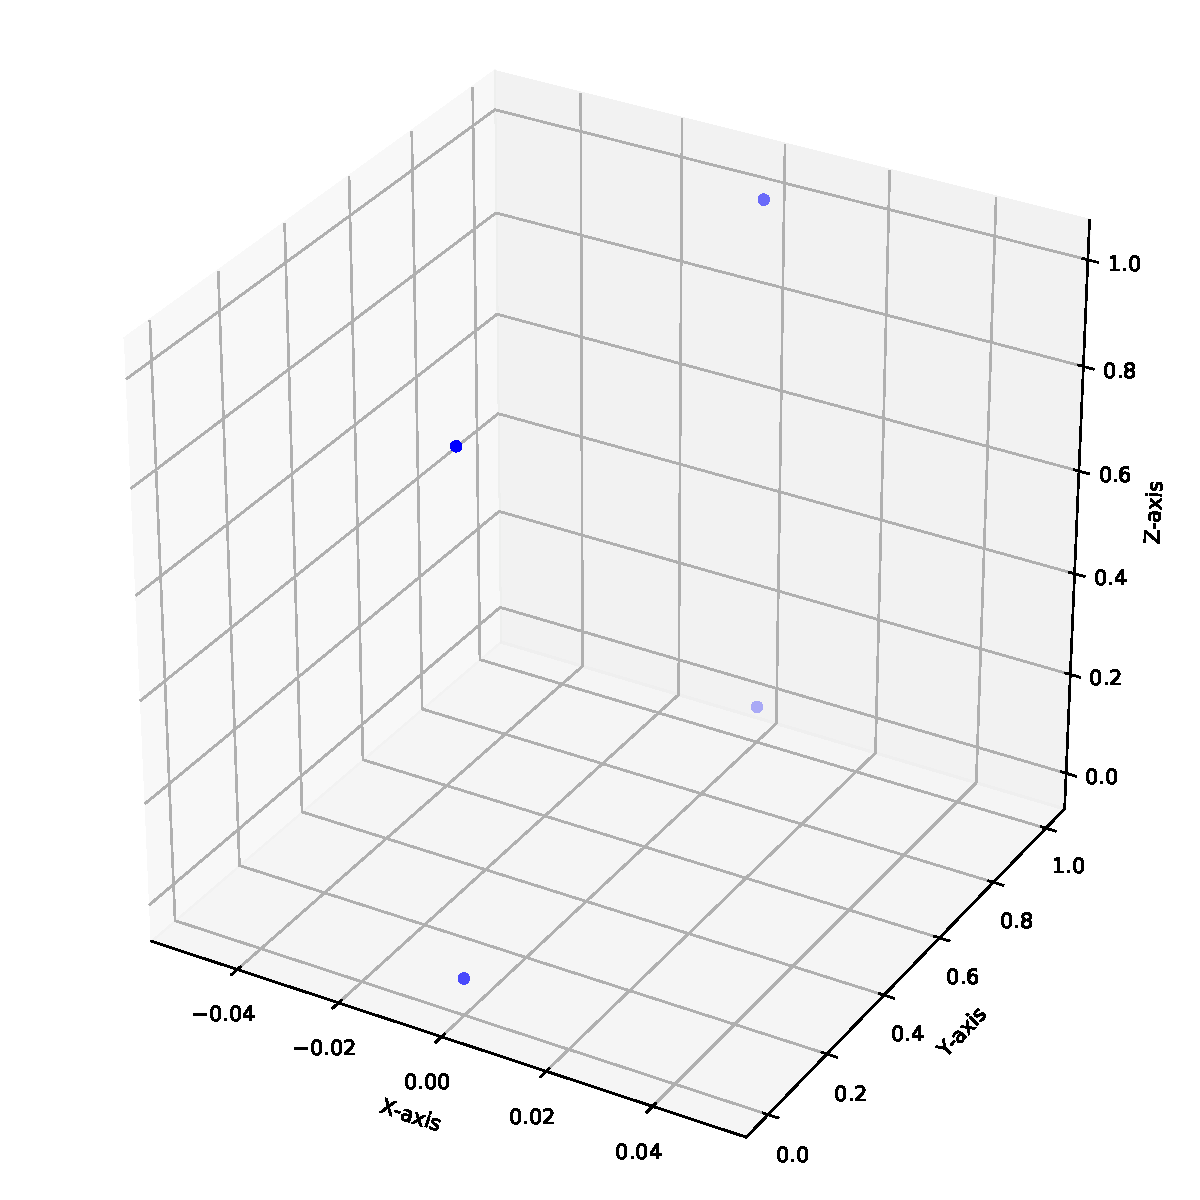
\includegraphics[width=0.4\textwidth]{./figure/ellipsoid_f1.pdf}
    \end{center}
    \caption{3D point cloud}\label{fig:}
\end{figure}
\subsection{}
\begin{figure}[htbp]
    \begin{center}
        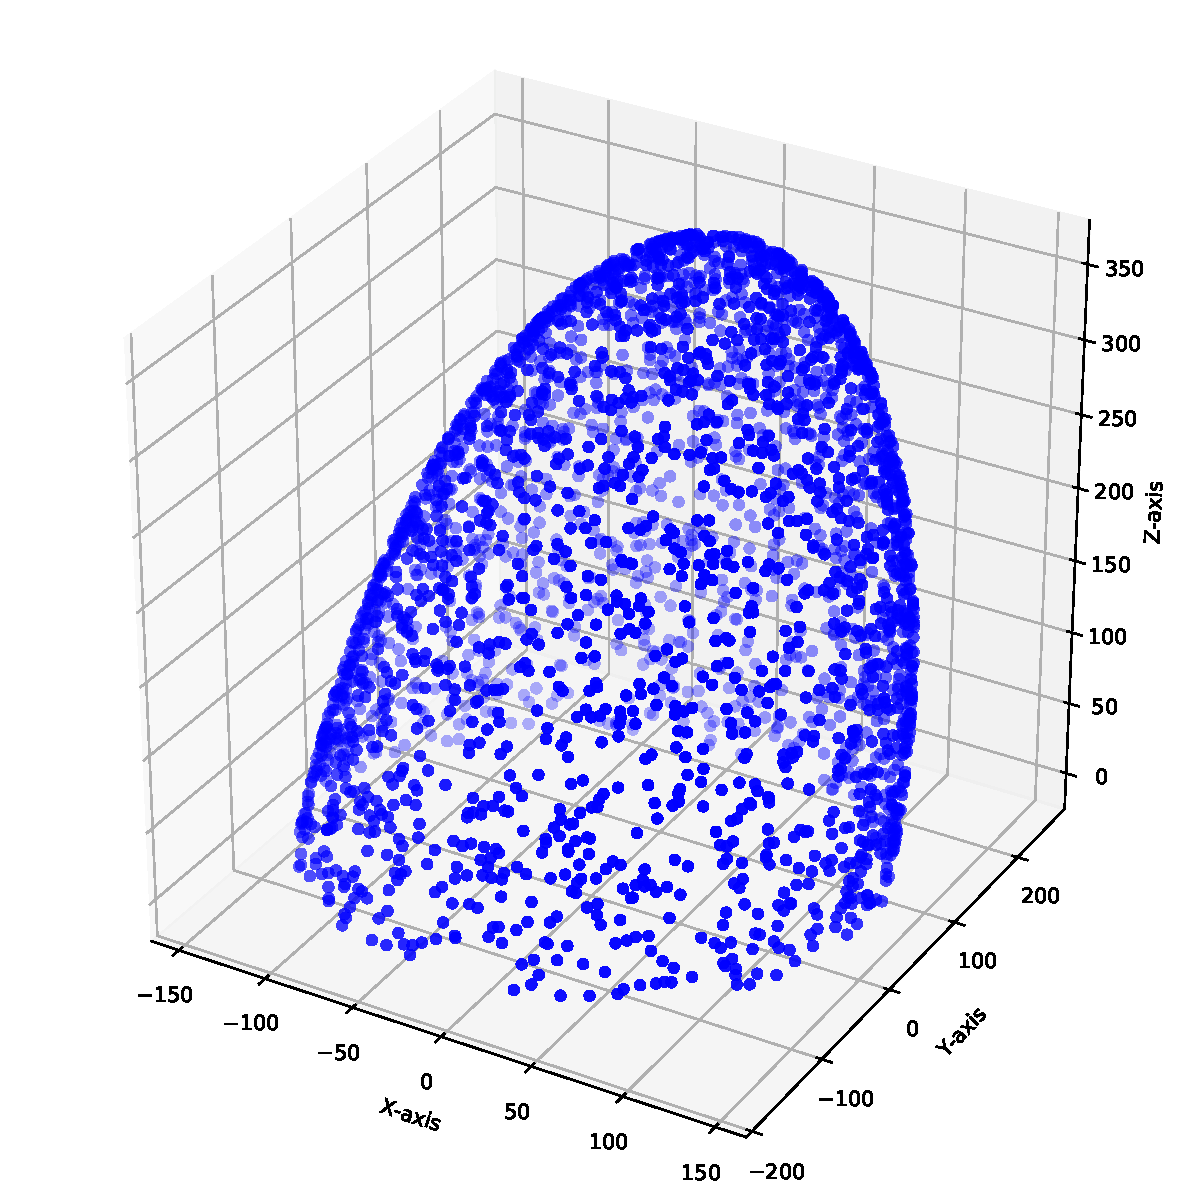
\includegraphics[width=0.4\textwidth]{./figure/ellipsoid_f2.pdf}
    \end{center}
    \caption{Half ellipsoid}\label{fig:}
\end{figure}
\clearpage
\section{Programming Problem: Linear Regression}
\subsection{}
By observing the output scatter plots, we pick these three relations as follows.
\begin{figure}[htbp]
    \begin{center}
        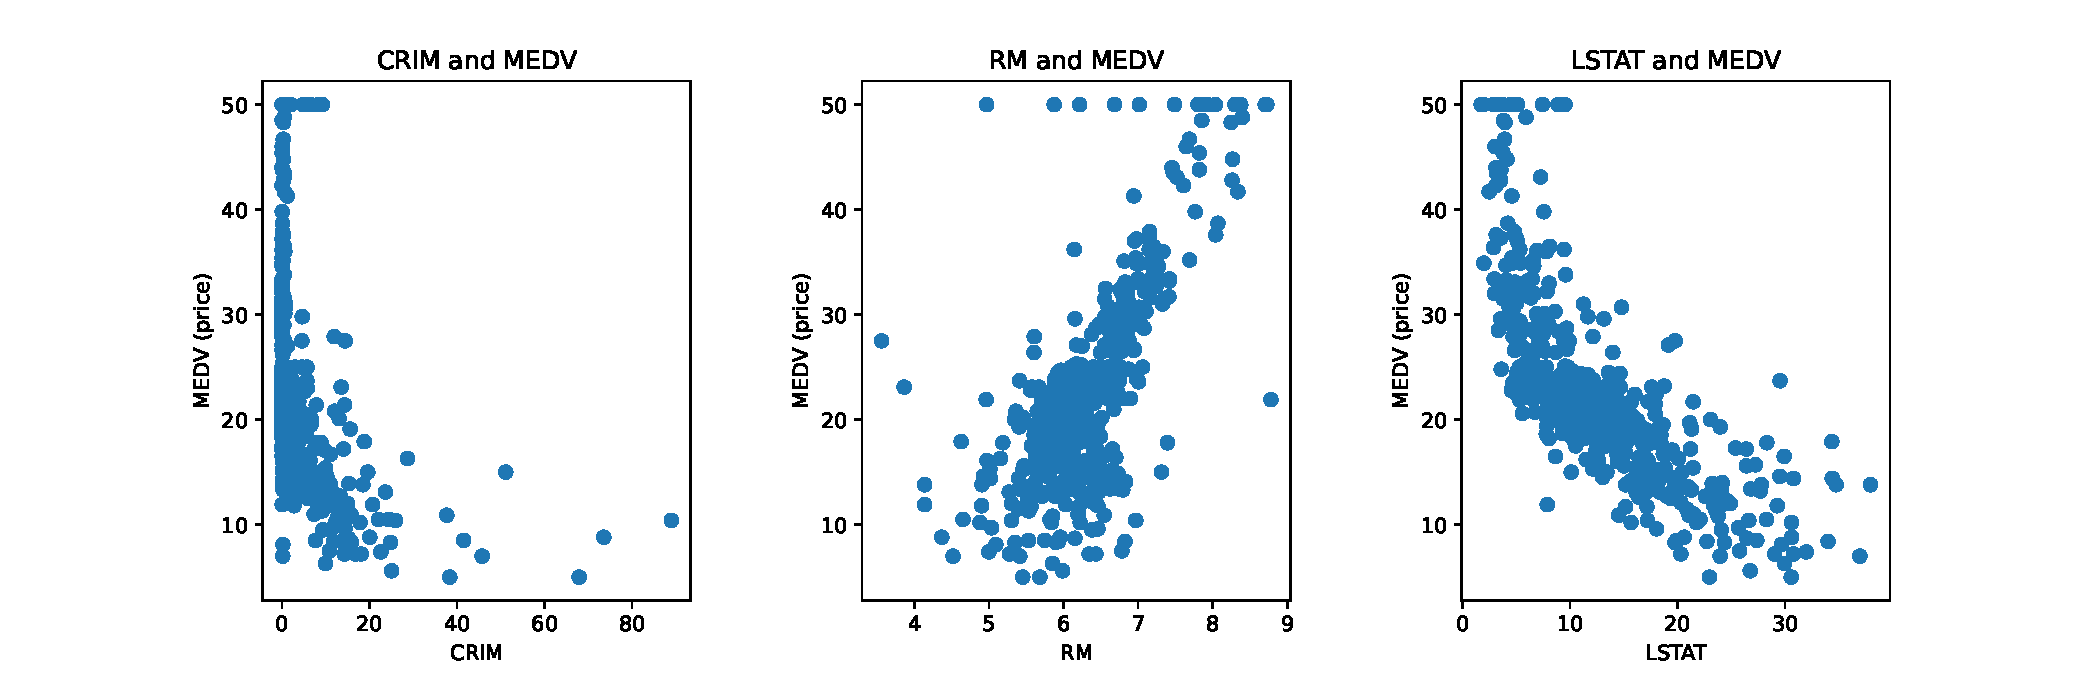
\includegraphics[width=0.7\textwidth]{./figure/linear_f2.pdf}
    \end{center}
    \caption{2D scatter plot for each feature}\label{fig:}
\end{figure}
\subsection{}
By the heatmap below, we can see that the top-3 features that are mostly linearly related to the ``MEDV" is ``LSTAT", ``PTRATIO", and ``RM". This is different as the ones in previous question.
\begin{figure}[htbp]
    \begin{center}
        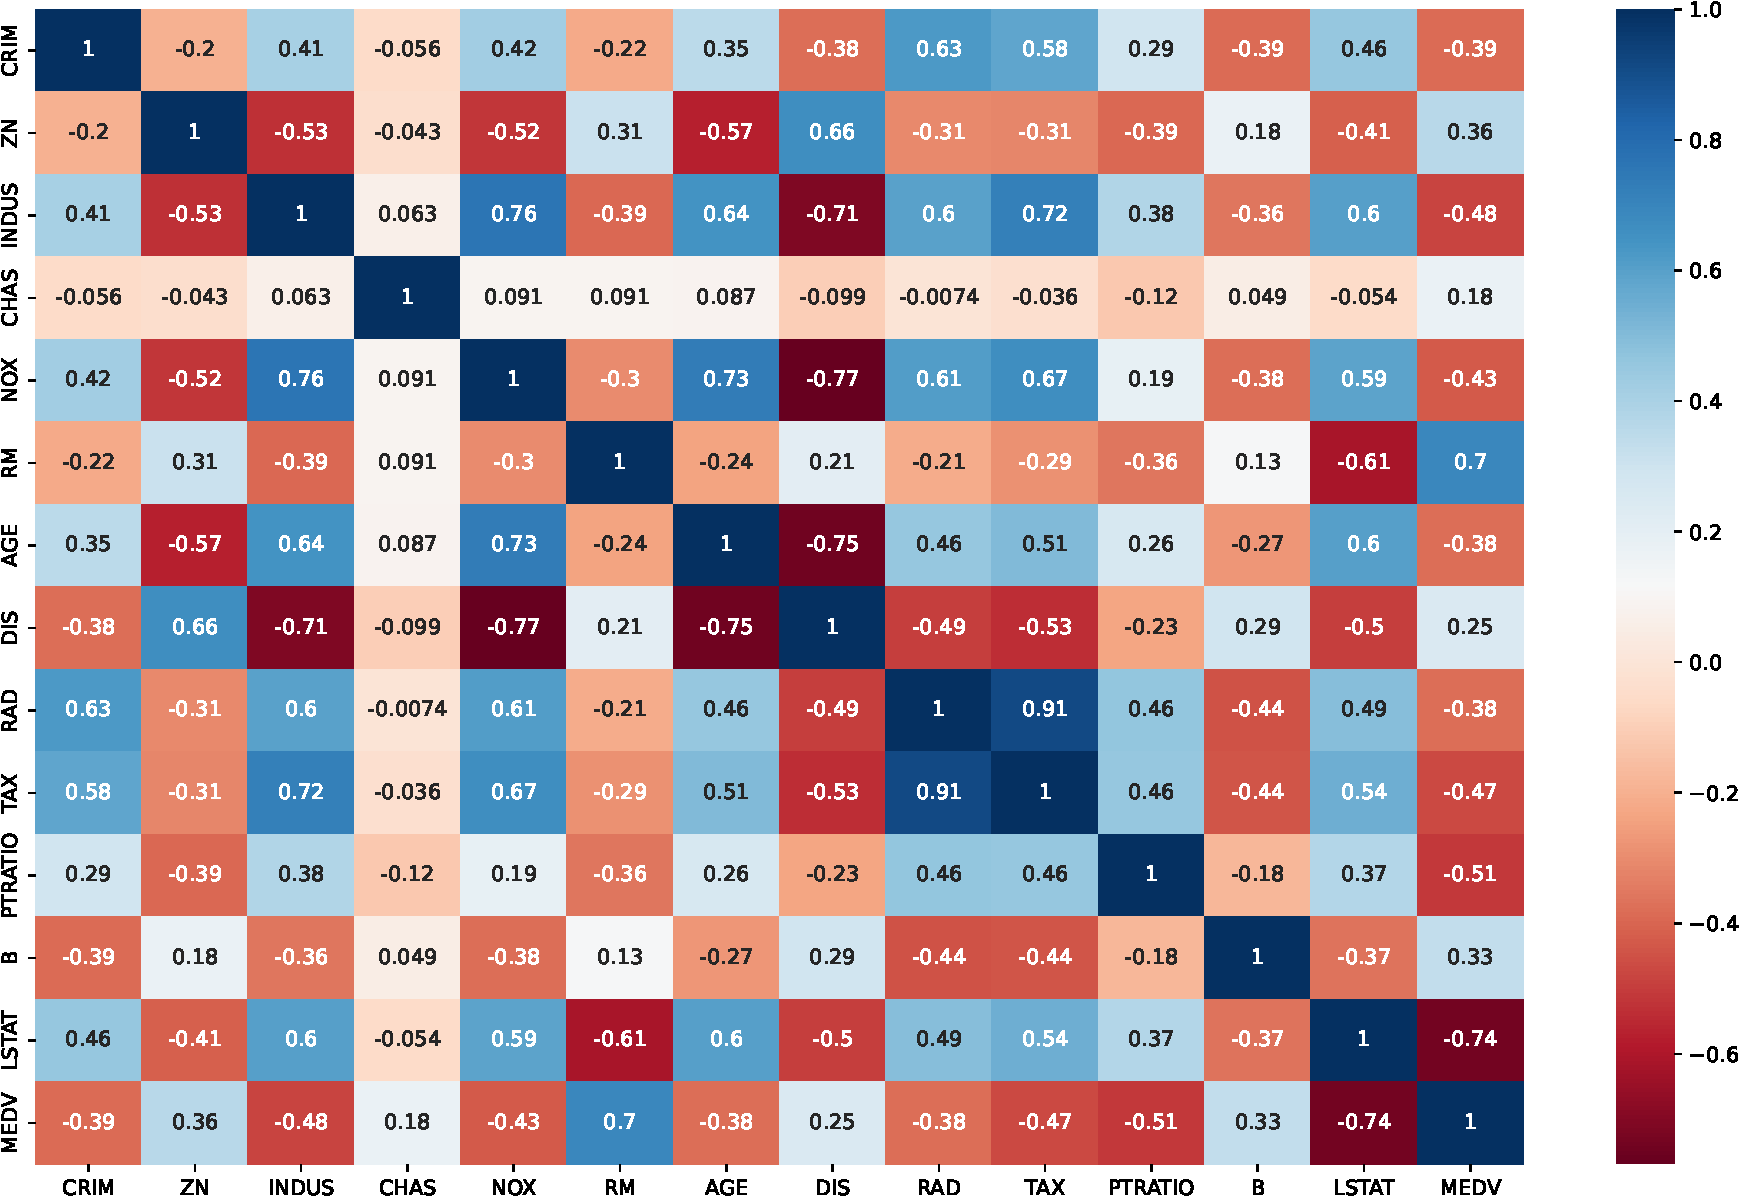
\includegraphics[width=0.75\textwidth]{./figure/correlation.pdf}
    \end{center}
    \caption{The heatmap of correlation matrix}\label{fig:}
\end{figure}
\clearpage
\subsection{}
\begin{table}[htbp]
    \begin{center}
\begin{tabular}{llrrrr}
\toprule
Feature & Coeff & Coeff\_eta\_15.0 & Coeff\_eta\_30.0 & Coeff\_eta\_45.0 \\
\midrule
 CRIM & -0.099324 & -0.100648 & -0.101157 & -0.101396 \\
 ZN & 0.052251 & 0.054632 & 0.056906 & 0.059028 \\
 INDUS & 0.004516 & 0.012958 & 0.016161 & 0.018062 \\
 CHAS & 2.957261 & 2.272783 & 1.854801 & 1.575958 \\
 NOX & 1.127938 & 0.457674 & 0.380824 & 0.343826 \\
 RM & 5.854198 & 5.728152 & 5.574767 & 5.424074 \\
 AGE & -0.014957 & -0.010094 & -0.006243 & -0.002772 \\
 DIS & -0.920844 & -0.896985 & -0.869514 & -0.842988 \\
 RAD & 0.159519 & 0.163084 & 0.164159 & 0.164232 \\
 TAX & -0.008934 & -0.008982 & -0.008988 & -0.008940 \\
 PTRATIO & -0.435674 & -0.406149 & -0.375560 & -0.345226 \\
 B & 0.014905 & 0.015518 & 0.015989 & 0.016406 \\
 LSTAT & -0.474751 & -0.484274 & -0.495622 & -0.506287 \\
\bottomrule
\end{tabular}
    \caption{The coeffcients correspondig to OLR and ridge regression}\label{tab:}
    \end{center}
\end{table}
\subsection{}
\begin{table}[htbp]
    \begin{center}
\begin{tabular}{llrr}
\toprule
 Model & RMSE\_test & RMSE\_train \\
\midrule
OLR & 5.209218 & 4.820627 \\
Ridge\_eta\_15 & 5.191204 & 4.826364 \\
Ridge\_eta\_30 & 5.187847 & 4.837923 \\
Ridge\_eta\_45 & 5.189540 & 4.852552 \\
\bottomrule
\end{tabular}
    \end{center}
    \caption{The RMSE on test and train dataset}\label{tab:}
\end{table}
From the table, we can see that as $ \eta $ increases, the RMSE on training dataset gets larger (we consider the ordinary linear regression as $ \eta = 0 $). However, we can notice that, on the test dataset, ridge regression do decreases the RMSE for proper eta. This is because ridge regression can prevent the model from overfitting to the training dataset, lead to a better performance on the test dataset.
\subsection{}
\begin{table}[htbp]
    \begin{center}
        \begin{tabular}{llrr}
\toprule
Model & RMSE\_test & RMSE\_train \\
\midrule
 Linear Regression & 5.494724 & 5.273362 \\
 Ridge Regression & 5.481155 & 5.275046 \\
\bottomrule
\end{tabular}
    \caption{The OLR and ridge regression by only using the top-3 features}\label{tab:}
    \end{center}
\end{table}
From this table we can notice that although we are just using the top-3 features, the RMSE is quite close to the RMSE which applying all features.
\clearpage
\section{Bonus: Locality Sensitive Hashing}
\subsection{}
In order to find exactly the nearest neighbor point in $ X $, we set $ c=1 $, which means the oracle will degraded into a simple oracle that tells us whether there are any point satisfying $ d(x,q)\leq r $. Thus, we can apply binary search, which is: every time we update the upper bound and lower bound of the search space by using the returned value of the oracle, and each time we set $ r $ as the middle point of the searching space. In this approach, we can have a time complexity at $ O(\log n) $.
\subsection{}
In this case, for given $ x_i $ and $ x_j $, we have $ d(x_i, x_j)\leq r $. And this indicates that $ x_i $ and $ x_j $ have at most $ r $ different digits and at least $ 0 $ different digits. As the function $ h $ mainly just pick one random digit from the number, we can see that for every two $ x $, there are $ \dfrac{m - r}{m} $ chances that they are the same value on the corresponding coordinate. Thus, $ p_1 = 1 - \dfrac{r}{m} $.\\
When $ d(x_i, x_j) \geq cr $, by following the same approach, we can see that there are at least $ cr $ digits that are not the same, thus, there are $ m - cr $ digits that are the same on the same coordinate. From this, we can deduce that in this case, there are $ \dfrac{m - cr}{m} $ chances that they are the same on the same coordinate. Which means $ p_2 = 1 - \dfrac{cr}{m} $
\subsection{}
In this occasion, we can see that $ g(x_i) $ can be considered as a intersection of k i.i.d. random variable. When $ d(x_i, x_j) \leq r$, $ p_1 = 1 - \frac{r}{m} $. When $ d(x_i, x_j)\geq cr $, $ p_2 = 1 - \frac{cr}{m} $. And when the function $ g(x_i) $ and $ g(x_j) $ have the same value, all the functions $ h_1(x_i), h_2(x_i)\cdots h_k(x_i) $ have the same values to $ h_1(x_j), h_2(x_j)\cdots h_k(x_j) $ correspondingly. Which means, when $ d(x_i, x_j)\leq r $, $ Pr(g(x_i)=g(x_j)) \geq p_1^k $. And when $ d(x_i, x_j)\geq cr $, $ Pr(g(x_i) = g(x_j))\leq p_2^k $
\subsection{}
In this case, all the function $ g $ are i.i.d., and here we only need there to be at least one b to satisfy the requirement,thus, we have $ Pr(\exists b, g_b(x_i) = g_b(x_j)) \geq 1 - ( 1 - p_1^k)^l $ when $ d(x_i, x_j) \leq r $. And we have $ Pr(\exists b, g_b(x_i) = g_b(x_j))\leq 1 - (1-p_2^k)^l $ when $ d(x_i, x_j) \geq cr $. 
\subsection{}
\begin{enumerate}
    \item According to problem 6.4, as $ d(x',q)\leq r $, we have $ Pr(\exists b, g_b(x')=g_b(q))\geq 1-(1-p_1^{\frac{\ln(n )}{\ln(1/p_2)}})^{n^{\frac{\ln(p_1 )}{\ln(p_2)}}} $\\
        In order to prove the inequality we desired, we only need to prove $ (1-p_1^{\frac{\ln(n )}{\ln(1/p_2)}})^{n^{\frac{\ln(p_1 )}{\ln(p_2)}}} \leq e^{-1} $. As we have $ p_1^{\frac{\ln(n) }{\ln{(1/p_2)}}} = p_1^{-\frac{\ln(n )}{\ln{(p_2)}}} = e^{-\frac{\ln(p_1)\ln(n)}{\ln(p_2)}} = (\frac{1}{n})^ {\frac{\ln(p_1)}{\ln(p_2)}} $. We can see that the original inequality is the same as:
        \begin{align*}
            \left(1 - \left(\frac{1}{n }\right)^{\frac{\ln(p_1)}{\ln(p_2)}}\right)^ {n ^ {\frac{\ln(p_1 )}{\ln(p_2)}}} \leq e^{-1}
        \end{align*}
        And by the inequality provided, we set $ k = n ^ {\frac{\ln(p_1 )}{\ln(p_2 )}} $, we can see that the inequality we desired is proved.
    \item According to Markov's inequality, we have $ P(X\geq a)\leq \frac{E(X)}{a} $, which means for the event, we have $ P(X\geq 4l) \leq \frac{E(X)}{4l} $. As $ d(x, q)\geq cr $, we have $ E(X) = n\cdot Pr(\exists b, g_b(x')=g_b(q)) \leq n\cdot (1-(1-p_2^{\frac{\ln(n) }{\ln(1/p_2)}})^l = n\cdot (1-(1-\frac{1}{n})^ {l}) \leq n\cdot (1-(1- \frac{l}{n}))= l $. Thus, $ \frac{E(X)}{4l}\leq \frac{l}{4l} = \frac{1}{4} $. Thus, we have $ P(X\leq 4l) = 1-P(X\geq 4l) \geq 1 - 1/4 = \frac{3}{4} $. Which means the second event happens with probability at least $ \frac{3}{4} $. 
    \item By the inequality we proved, we can see that we have the lower bound for each two events. As the two events are independent, we can see that the lower bound that both event happens is $ \frac{3}{4} (1-e^{-1}) $.
\end{enumerate}
\end{document}
